\scanpage{9}
\mspage{2}
i.e. on a, pour \(\deleted{x}\xi\in J_n(n')\) i.e. \(x\in J_n,\ \tau_n(x)=n'\)
\[
 u_\xi(d_{n'})=\xi .
\]
\deleted{De} plus, \unsure{fort|faut|fut} encore,
% The brace has a downward central notch and a long rising return on its right.
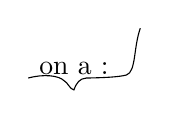
\begin{tikzpicture}[baseline=(a.base),x=1em,y=1em]
 \node[inner sep=0] (a) at (0,0) {on a :};
 \draw (-1.65,-.35) .. controls (-1.1,-.2) and (-.55,-.25) .. (-.35,-.45)
 .. controls (-.23,-.5) and (-.15,-.75) .. (0,-.78)
 .. controls (.1,-.52) and (.2,-.37) .. (.45,-.35)
 .. controls (1.0,-.34) and (1.6,-.32) .. (1.9,-.24)
 .. controls (2.25,-.12) and (2.15,.75) .. (2.4,1.45);
\end{tikzpicture}
\inserted{\(u_\xi\) induit un isom}
\(J_{n'}\xrightarrow{\overset{u_\xi}{\sim}}(J_n)_{\leq\xi}\)

Lorsque \(n'=n\), on a \(J_{n,n}=\{d_n\}\), et
\[
 u_{d_n}=\mathrm{id}_{J_n}
\]

La connaissance de \(\mathbb N,\ (J_n)_{n\in\mathbb N},\ (\tau_n)_{n\in\mathbb N},\
(\rho_{n,n'})_{\substack{(n',\deleted{\unsure{n'|m}}n)\in\mathbb N\times\mathbb N\\ n'\leq n}}\) permet de reconstituer \deleted{à peu de \unsure{chose|choses} près} \deleted{essentiellement \unsure{la|le} sous-catégorie pleine}\inserted{la catégorie} \(M\), à \deleted{il} équiv près, il manque encore une \deleted{\unsure{description|descripteur}} \inserted{condition} pour composer les hom ``standart entre les \(J_n\), i.e ceux provenant des \(J_{n',n'}\). \deleted{Donc} On considère une situation
\diagram{\begin{tikzcd}[ampersand replacement=\&,column sep=.8em,row sep=small]
 \& \& \eta \&[1.3em] \& \xi\\[-.8em]
 \& \& \rotatebox{-90}{\(\in\)} \& \& \rotatebox{-90}{\(\in\)}\\
 J_{n''}\arrow[rr,"u^{n'}_{\eta}"] \& \& J_{n'}\arrow[rr,"{u_\xi^n}"{inner sep=0pt,yshift=-1.1ex}] \& \& J_n\\
 n'' \& \leq \& n' \& \leq \& n
\end{tikzcd}}
% Both membership arches open down. The second shaft is longer; its xi descender crosses it.
on doit avoir
\[
 u_\xi^n\,u_\eta^{n'}=u_{\deleted{\unsure{a|\xi}}\zeta}^{n}
 \qquad\text{où}\quad \zeta=u_\xi^n(\eta)=
 (u_\xi^n\,u_\eta^{n'})(d_{n''})
\]
qui exprime la \deleted{\unsure{stabilité|composition|stabilis}} stabilité de la notion d'hom admissible \unsure{entre.|entre} \(J_n\) par composition.

\deleted{Il est évident que la \unsure{catég|caté}} \inserted{Soit \(M_0\) la catégorie définie par}
\[
 \mathrm{Ob}\,M_0=\mathbb N,\quad \mathrm{Hom}_{M_0}(n',n)=
 \left\{\begin{aligned}
 &\varnothing\ \text{si }n'\nleq n\\
 &\text{ens. des hom. admissibles}\\
 &\qquad J_{n'}\to J_n\quad\text{si }n'\leq n
 \end{aligned}\right.
\]
% archive sheet number: 8
